\documentclass{article}
\usepackage{iclr2021,times}
\iclrfinalcopy % Camera ready version!

\usepackage[utf8]{inputenc}
\usepackage[T1]{fontenc}

\usepackage[hyphens]{url}
\usepackage{hyperref}
\usepackage{graphicx}
\hypersetup{
    colorlinks,
    citecolor=blue,
    filecolor=blue,
    linkcolor=blue,
    urlcolor=blue,
}
\usepackage{algorithm}
\usepackage{algorithmic} 

\usepackage{natbib}
\setcitestyle{authoryear,open={(},close={)}}

\usepackage{amsmath,amssymb}
\usepackage{makecell}
\usepackage{chngcntr} % make figure numbering in appendix work

\usepackage{caption}
% Small captions
\captionsetup[figure]{font=small,labelfont=small}

%%% SPACE-REDUCING HACK 1/2
% Reduce spacing around floats 
\setlength{\floatsep}{8pt plus 4pt minus 4pt}
\setlength{\textfloatsep}{8pt plus 4pt minus 3pt}

\usepackage{xcolor}
\bibliographystyle{iclr2021}


\title{Planetary Nebulae Classification from Limited Labeled Dataset
\\ {\small Final Report for \href{https://www.cs.tufts.edu/cs/152L3D/2024f}{CS 152 L3D at Tufts in Fall '24}}
}
\author{Joseph Hadidjojo \And Tung Pham \And Arman Muratbayev
}

\begin{document}

\maketitle


% {\color{red} \textbf{Instructions:} \url{https://www.cs.tufts.edu/cs/152L3D/2024f/final_report.html}}

Sharing permission statement:
\\ {\small Instructors can share this report to future students of similar classes}

\section{Introduction}

% \subsection{Prediction Task}
% TODO Paragraph 1: What's the prediction task?

Planetary nebulae (PNe) represent a late stage in the life cycle of medium-mass stars, marked by glowing elliptical objects of ionized gas. Accurately distinguishing true PNe from visually similar non-PNe objects is challenging due to the overlap in visual characteristics (such as shape and luminosity) with other types of nebulae and celestial bodies. Given this context, this work aims to classify True vs Rejected PNes from 3-channel (RGB), 224 x 224 deep-space images of glowing, elliptical space objects.

\subsection{Overall Goal}
% TODO Paragraph 2: What's your overall goal?

This study aims to build upon prior work by \cite{awangiskandar2020}, that first applied a Transfer Learning (Linear Probing) approach towards Planetary Nebulae classification (achieving over 80\% prediction accuracy). Our objectives are twofold: first, to reproduce the original results as a benchmark, and second, to explore whether more advanced methods—such as Linear Probing with Fine-Tuning (LP-FT) and MixMatch Pseudo-Labeling—can push this accuracy even higher. This work is exciting as it not only attempts to validate pioneering Transfer Learning techniques within the Astrophysical context, but also tests innovative adaptations that may set new standards in identifying PNes with greater precision. Positive results from this study may motivate Astronomers to more readily explore and adopt ML techniques during deep-space explorations and analysis. From the ML perspective, this work presents performance of ImageNet-based Transfer Learning and MixMatch Semi-Supervised Learning methods on a mostly never-before-seen, “Low-Resolution” dataset.


\subsection{Methods Summary}
% TODO Paragraph 3: Introduce the methods you'll study.

This work leverages Transfer Learning, where models pre-trained on large datasets (ImageNet) are adapted to specialized tasks, enhancing performance with minimal labeled data (\cite{pan2010survey}). The primary methods include Linear Probing (LP), which retrains only the final layer of the model, and  Linear Probing with Fine-Tuning (LP-FT),  which hopes to further improve accuracy by fine-tuning deeper layers (\cite{kumar2022lpft}). Additionally, we leverage the Semi-Supervised Learning method known as pseudo-labeling (\cite{lee2013pseudo}), specifically MixMatch (\cite{berthelot2019mixmatch}), to generate ``soft'' labels for unlabeled data, allowing the model to train on a larger, unlabeled dataset. Due to the nature of our dataset, we will be performing color properties augmentation (colorspace, brightness, contrast) instead of physical augmentation (rotational, translational, cropping) for our MixMatch implementation.

While LP is computationally efficient, its adaptability is limited, potentially capping model performance. LP-FT, in contrast, offers greater flexibility and accuracy by adjusting multiple layers, though it increases training complexity and the risk of overfitting if not carefully tuned. In contrast, Pseudo-labeling attempts to boost accuracy further by including additional data, but it can introduce label noise, especially when initial predictions are uncertain. This work will attempt to balance these trade-offs---accuracy, computational costs, and training stability---to identify the most effective approach for PNe classification.

\subsection{Hypothesis}
% TODO Paragraph 4: Specific hypothesis

The hypothesis for this experiment is that a \textbf{combination of Linear Probing and Fine-Tuning (LP-FT) on a pre-trained model will outperform independent MixMatch Pseudo-labeling in classification accuracy of True or Rejected PNe}. 

Our hypothesis is primarily grounded in MixMatch's dependence on consistency regularization across various input perturbations, and in the potential of LP-FT to better align with the demands of a specific target task or domain. Given the nature of our dataset (low-resolution images of deep-space elliptical objects, often procured by cropping certain regions of interest from original deep-space image), we hypothesize that the MixMatch method might not be able to extract enough discriminative representations of True PNes from image transformations/augmentations alone to pseudo-label the unlabeled dataset effectively. In contrast, the Fine-Tuning phase of LP-FT is widely known for its capability to optimally learn the nuanced requirements of a target task. However, should MixMatch prove to be able to pseudo-label effectively, we acknowledge that it might be able to outperform the LP-FT model due to the fact that it will be able to leverage the unlabeled portion of our dataset which LP-FT would not.

Other approaches commonly used for learning with limited labeled data, such as Contrastive Self-Supervised methods, may be less appropriate in this context. As an example, SimCLR, which relies on data augmentations and contrastive pairs, may struggle with low-resolution PNe images and noise from nearby bright stars, leading to potentially learning artifacts rather than meaningful features. 

\section{Methods}

\subsection{Transfer Learning using LP-FT}

\textbf{Linear Probing with Fine-Tuning (LP-FT)} builds upon the principles of Transfer Learning by adapting pre-trained models (trained on large-scale datasets like ImageNet) to domain-specific tasks with limited labeled data. This method follows the approach as established by \cite{kumar2022lpft} and involves two stages: first, \textit{Linear Probing}, followed by \textit{Fine-Tuning}. Linear Probing serves as a computationally efficient baseline by retraining only the final fully connected layer of the model while keeping all other layers frozen. This approach leverages the general features learned from pre-trained dataset and aligns them with the target task while minimizing computational costs.

Our classification task involves distinguishing between True and Rejected planetary nebulae (PNe), making it a binary classification problem. The pre-trained \textit{DenseNet-201} model takes $224 \times 224$ images as input and outputs a single probability $\hat{y} \in [0, 1]$, representing the likelihood of an image being classified as True PNe. To adapt the DenseNet-201 model for this binary classification task, the final classification layer is replaced with a single-output layer with a sigmoid activation function:
\[
\hat{y}_i = \frac{1}{1 + e^{-z_i}},
\]
with $z_i$ being the model’s raw output before activation. Binary cross-entropy loss is used to optimize predictions of the final classification layer:
\[
\mathcal{L}_{BCE} = -\frac{1}{N} \sum_{i=1}^N \left[ y_i \log(\hat{y}_i) + (1 - y_i) \log(1 - \hat{y}_i) \right],
\]

where $N$ is the batch size and $y_i$ is the true label ($y = 1$ for True PNe, $y = 0$ for Rejected PNe).


Fine-Tuning extends this approach by gradually unfreezing selected layers of the model. During this process, both the final classification layer and the selected pre-trained layers are optimized using a regularized binary cross-entropy loss:
\[
\mathcal{L} = \mathcal{L}_{BCE} + \frac{\lambda}{2} \|\theta_{FT}\|^2,
\]
where $\lambda$ is the regularization strength and $\theta_{FT}$ represents the parameters of the fine-tuned layers. The regularization term, also known as L2 regularization, discourages large parameter updates to preserve the generalizable knowledge encoded in the pre-trained model. In this work, we explore unfreezing the top 3 and 5 layers of the model respectively.


Our implementation is built upon the starter code provided by Prof. Michael C. Hughes for Homework 1 of the 'Learning with Limited Labeled Data' course at Tufts University (\cite{hughes_hw1_2024}). This implementation leverages the \textit{PyTorch} deep learning framework (\cite{paszke2019pytorch}), with the pre-trained DenseNet-201 architecture sourced from the \textit{pytorchcv library}. Parameter updates during all three phases (pre-training, Linear Probing and Fine Tuning) were done using the \textit{Adam optimizer}, which adjusts learning rates dynamically based on gradient estimates, ensuring stable convergence and efficient updates. Fine tuning layers customization were controlled through PyTorch’s parameter freezing functionality, enabling selective gradient updates only for the designated layers.

The motivation for LP-FT lies in balancing performance improvement and computational cost. Linear Probing is computationally efficient but limited in its ability to adapt to the dataset's unique characteristics. Fine-Tuning offers greater flexibility and enables the model to refine its feature representations for the target domain. By carefully implementing these strategies, LP-FT aims to optimize the model’s ability to classify True and Rejected PNe, leveraging the strengths of pre-trained models and addressing the challenges posed by the specialized dataset.

\subsection{Semi-Supervised Learning using MixMatch}

\textbf{MixMatch} is a semi-supervised learning method that leverages unlabeled data to reduce reliance on large labeled datasets. It augments both labeled and unlabeled data, creating multiple augmented versions of each sample. Pseudo-labels are then generated for the unlabeled based on the model's predictions. These predictions are then averaged across the augmented versions to produce more stable pseudo-labels, which are further refined using a sharpening technique to increase confidence in the predictions. By combining these steps, MixMatch captures patterns from both labeled and unlabeled data, improving generalization and predictive performance

A key baked-in feature of MixMatch is \textbf{MixUp}, an integrated data augmentation/mixing technique to enhance generalization by creating interpolated training examples. Specifically, MixUp generates new samples by linearly combining pairs of data points and their corresponding labels. Given two samples \((x_i, y_i)\) and \((x_j, y_j)\), MixUp produces a new sample \((\tilde{x}, \tilde{y})\) as:

\[
\tilde{x} = \lambda x_i + (1 - \lambda) x_j, \quad \tilde{y} = \lambda y_i + (1 - \lambda) y_j,
\]

where \(\lambda\) is drawn from a Beta distribution \(\text{Beta}(\alpha, \alpha)\), with \(\alpha > 0\) controlling the degree of interpolation.
In MixMatch, MixUp is applied not only to the labeled data but also to the unlabeled data with pseudo-labels.
For each feature and its corresponding label, another pair was selected at random for the operation.
This regularization encourages the model to behave linearly between samples, improving its robustness and ability to generalize, particularly in the semi-supervised learning setting.

The loss function is a combination of the supervised learning binary cross-entropy loss on the labeled data between the prediction and the actual labels, and a $L_2$ loss between the prediction and the guess labels on the unlabeled data:
\[
    \mathcal{L}_{\mathcal{X}} = \frac{1}{|\mathcal{X}'|} \sum_{x,p \in \mathcal{X}'} H(p, p_{\text{model}}(y|x;\theta))
\]

\[
    \mathcal{L}_{\mathcal{U}} = \frac{1}{L|\mathcal{U}'|} \sum_{u,q \in \mathcal{U}'} \|q - p_{\text{model}}(y|u;\theta)\|_2^2
\]

\[
    \mathcal{L} = \mathcal{L}_{\mathcal{X}} + \lambda_{\mathcal{U}}\mathcal{L}_{\mathcal{U}}
\]

where $\mathcal{L}_{\mathcal{X}}$ represents the supervise learning loss on the labeled data, $H$ is the cross-entropy function, and $\mathcal{L}_{\mathcal{U}}$ represents the $L_2$ loss on the unlabeled data.

Our MixMatch implementation is adapted from a MixMatch implementation by YU1ut (available on GitHub: \cite{yu1ut_mixmatch_pytorch}) and leverages the \textit{PyTorch} deep learning framework (\cite{paszke2019pytorch}), with a ResNet50 architecture (sourced from the \textit{pytorchcv library}) pretrained on the ImageNet dataset as the initial backbone. The final classification of this ResNet50 model is replaced with single-output layer in the same way as our LP method. Given the nature of our dataset images, we leverage PyTorch's ColorJitter feature to apply color transformations instead of typical rotational or translational augmentations. Parameter updates during all phases were done using the \textit{Adam optimizer}.

Compared to other state-of-the-art techniques, MixMatch unifies the core principles of semi-supervised learning---entropy minimization, consistency regularization, and generalization---into a single, cohesive loss formulation. This unified framework allows MixMatch to achieve state-of-the-art performance, significantly reducing error rates while maintaining a streamlined and computationally efficient design (\cite{berthelot2019mixmatch}). Notably, its flexibility enables seamless adaptation to diverse model architectures and datasets, demonstrating broad applicability across a range of tasks. We believe that this adaptability makes MixMatch particularly suitable for limited-labeled dataset settings, and we leverage its strengths to address our target task of classifying True Planetary Nebulae.

\section{Data and Experimental Plan}

\subsection{Dataset description}
To create our dataset, we scraped Optical Images of possible PNes from the SuperCOSMOS Sky Survey (SSS), as compiled and hosted by the \textbf{\textit{H}}ong Kong/Australian \textbf{\textit{A}}stronomical Observatory/ \textbf{\textit{S}}trasbourg Observatory \textbf{\textit{H}}-alpha Planetary Nebula (HASH-PN) research platform database (which we will from here on refer to as HashDB). HashDB compiles over 30,000 deep-space images of possible or suspected PNes, of which only a fraction of them are labeled as "True PNe" (independently confirmed to be a Planetary Nebulae). The remaining images are either unlabeled (indicating "Possible PNe") or labeled as "Rejected PNe" (independently confirmed to be other types of Nebulae) (\cite{parker2016hash}). These images are also of different modalities, and are grouped based on the equipment and method used to capture the respective images (e.g., Optical, Quotient, WISE342).

\begin{table}[h!]
\centering
\begin{tabular}{|c|c|c|c|c|c|}
\hline
\textbf{ID} & \textbf{Name} & \textbf{DRAJ2000} & \textbf{DDECJ2000} & \textbf{Image} & \textbf{Label} \\ \hline
32280 & Dr 21 & 350.95788 & 45.28179 & 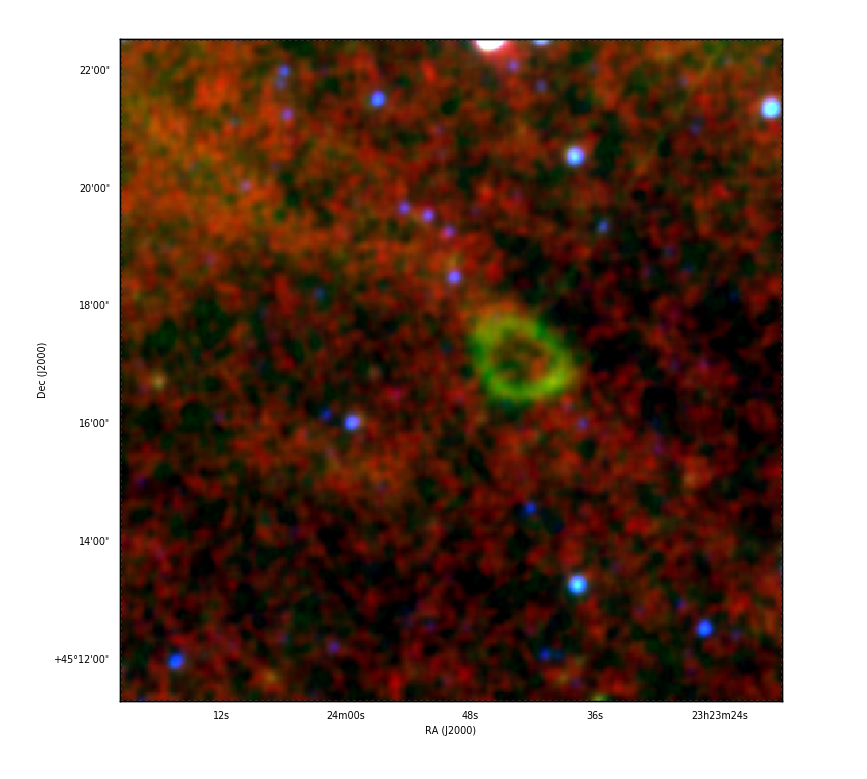
\includegraphics[width=1in]{32280_wise432_rgb.png} & True PNe \\ \hline
17907 & NGC 16 & 111.58614 & -34.2072 & 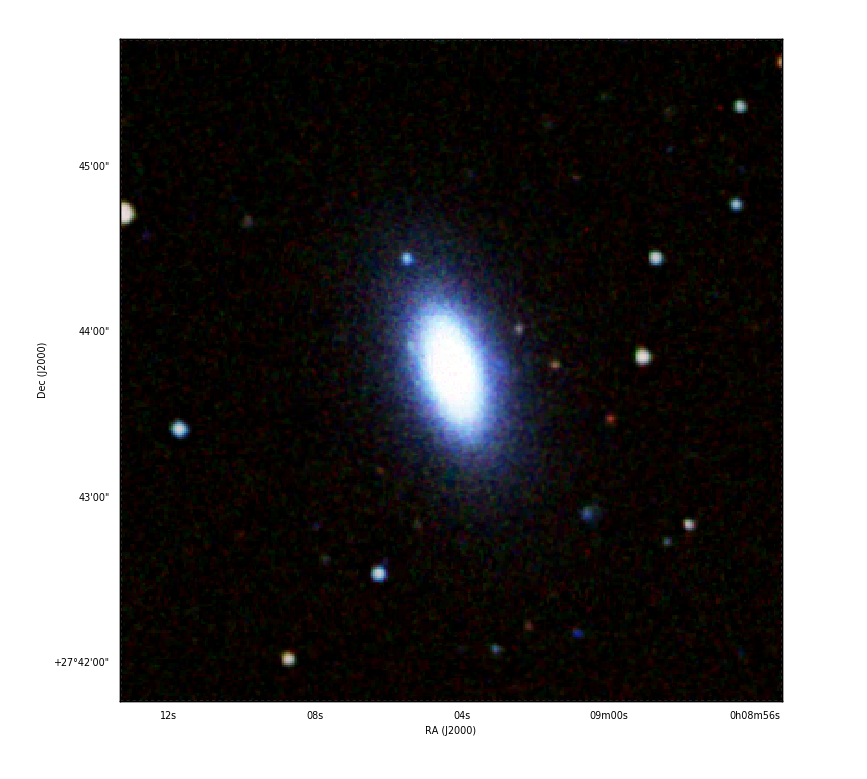
\includegraphics[width=1in]{17907_sss_irb2.png} & Rejected PNe (galaxy) \\ \hline
\end{tabular}
\caption{Subsample of HashDB dataset}
\end{table}

\subsection{Splitting Data to train/tune/assess generalization.}

% As mentioned previously, our dataset was built using 1,000 sub-samples of the HashDB 'Optical' group subset.
Our dataset consists of 1,000 sub-samples from the HashDB 'Optical' group subset, which are 3-channel RGB images in nature. The first 500 of this dataset are evenly sampled from both the "True PNe" and "Rejected PNe" labeled images to create an evenly distributed labeled dataset for use in our Baseline and LP-FT method. The remaining 500 are sampled from HashDB's unlabeled pool to create an unlabeled dataset for our Pseudo-labeling method. While we acknowledge that this might not be the best representation of 'True' vs. 'Rejected' PNes in space, we also note the immense scale of the galaxy and the lack of knowledge in the distribution of PNes vs other Nebulaes. With this in mind, we constructed our dataset with the intention of mitigating possible complications and uncertainties that we currently have little knowledge of. \footnote{We reached out to the original authors (\cite{awangiskandar2020}) to request access to their existing dataset. However, we only received their response in early December, which was too late for our timeline, hence we proceeded with our work using our own curated dataset as described.}

Both labeled and unlabeled datasets will be split into a Train/Test/Validate set for the purpose of training, hyperparameter tuning, and assessing generalization respectively. The split will be done in an 8:1:1 ratio, following the splits originally defined by \cite{awangiskandar2020}, but with an added emphasis on preventing data leakage which was not originally discussed in that paper. This was achieved through leveraging the included DRAJ2000 and DDEC2000 values in the dataset, which represent the object's coordinates in space. These coordinates will be used to ensure that no two images with the same coordinates exist across the different data split. 

\subsection{Performance metric}
For this experiment, the primary performance metric will be \textbf{classification accuracy}, which measures the proportion of PNe images correctly classified as True or Rejected. This metric is appropriate as the primary goal of the experiment is to maximize correct identifications of PNe types. Precision and Recall were initially considered as candidate additional metrics as well but were later deemed redundant given the deliberately balanced nature of the dataset.

\subsection{Training and hyperparameter tuning plan}

For each training phase of all three methods, we perform mini-batch gradient descent with PyTorch's Adam optimizer implementation (\cite{paszke2019pytorch}) with a fixed learning rate. Each training phase proceeds for up to 100 epochs. After every epoch, we record the cross-entropy loss on the validation set. If this value plateaus for 25 consecutive epochs, we stop the training phase early.

Both supervised and semi-supervised learning can be quite sensitive to hyperparameters.
Our hyperparameter tuning plan includes tuning both shared hyperparameters (learning rate) and unique hyperparameters.
For baseline and LP-FT, we sweep through 3 different learning rates as well as model complexity (L2 regularization strength $\lambda$). For the Fine-Tuning phase, we explicitly reduced the learning rates by a factor of 10. Table \ref{table:lpft-search} presents a summary of our LP-FT hyperparameter search space.

\begin{table}[!ht]
    \centering
    \begin{tabular}{|c|c|}
    \hline
    \textbf{Hyperparameter} & \textbf{Search Space} \\ \hline
    LP learning rate & [0.001, 0.0001, 0.0001] \\ \hline
    FT learning rate & [0.0001, 0.00001, 0.000001] \\ \hline
    $\lambda$ & [0, 0.1, 0.01] \\ \hline
    \end{tabular}
    \caption{LP-FT Hyperparameter Search Space}
    \label{table:lpft-search}
\end{table}

For MixMatch, we search through $T$ (sharpening temperature), $\alpha$ (Beta-distribution parameter for use in MixUp), and $\lambda_u$ (unlabeled loss weight).
\cite{berthelot2019mixmatch} recommends starting with $T = 0.5$, $\alpha = 0.75$ and $\lambda_u = 100$ as a starting point. It should also be noted that Berthelot et al. found that most of MixMatch’s hyperparameters can be fixed and do not need to be tuned on a per-experiment or per-dataset basis. Additionally, we used $K = 2$ where only 2 sets of augmentations are applied, and used the space described in Table \ref{table:mixmatch-search} in our hyperparameter search.

\begin{table}[!ht]
\centering
\begin{tabular}{|c|c|}
\hline
\textbf{Hyperparameter} & \textbf{Search Space} \\ \hline
learning rate & [0.0001, 0.00001] \\ \hline
$\lambda_u$ & [10, 30, 50, 80, 100] \\ \hline
$T$ & [0.5, 1.0] \\ \hline
$\alpha$ & [0.5, 0.75, 1.0] \\ \hline
\end{tabular}
\caption{MixMatch Hyperparameter Search Space}
\label{table:mixmatch-search}
\end{table}



\section{Results}

\begin{table}[!ht]
    \centering
    \begin{tabular}{| l | c |}
    \hline
    \textbf{Method} & \textbf{Classification Accuracy} \\ \hline
    Baseline LP (\cite{awangiskandar2020}) & 86.0 \\ \hline
    Baseline LP (Ours) & 88.0 \\ \hline
    LP-FT, 3 top-layers (Ours) & 84.4 \\ \hline
    LP-FT, 5 top-layers (Ours) & 84.0 \\ \hline
    Mix-Match Pseudo-labeling (Ours) & 78.0 \\ \hline
    \end{tabular}
    \caption{\textbf{Evaluation Results based on Test Dataset}}
    \label{table: test_acc_table}
\end{table}

\begin{figure}[!ht]
    \centering
    \begin{tabular}{c c}    
    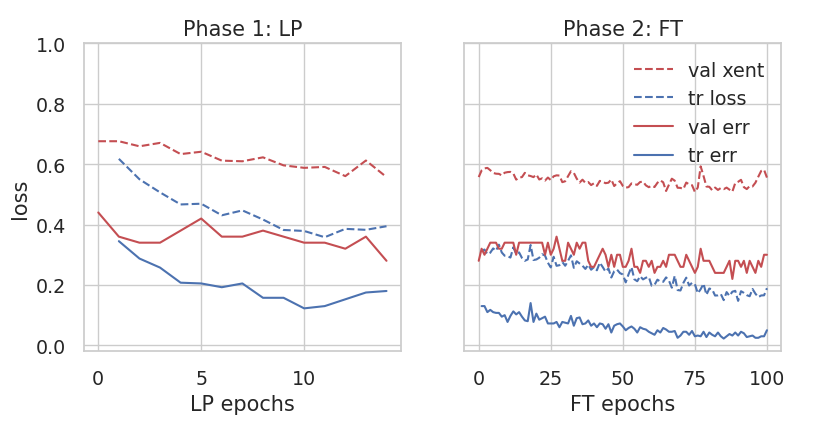
\includegraphics[width=0.45\textwidth]{lp_ft_3.png}
    &
    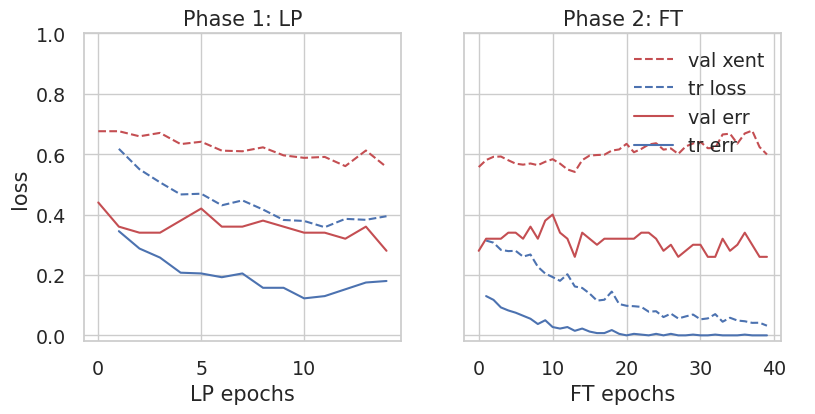
\includegraphics[width=0.45\textwidth]{lp_ft_5.png}
    \end{tabular}
    \caption{\textbf{Diagnostic Learning Plots for LP-FT: Top 3 (left) and 5 (right) Layer Fine Tuning}}
    \label{figure: diag_plot_lpft}
\end{figure}

\begin{figure}[h!]
    \centering
    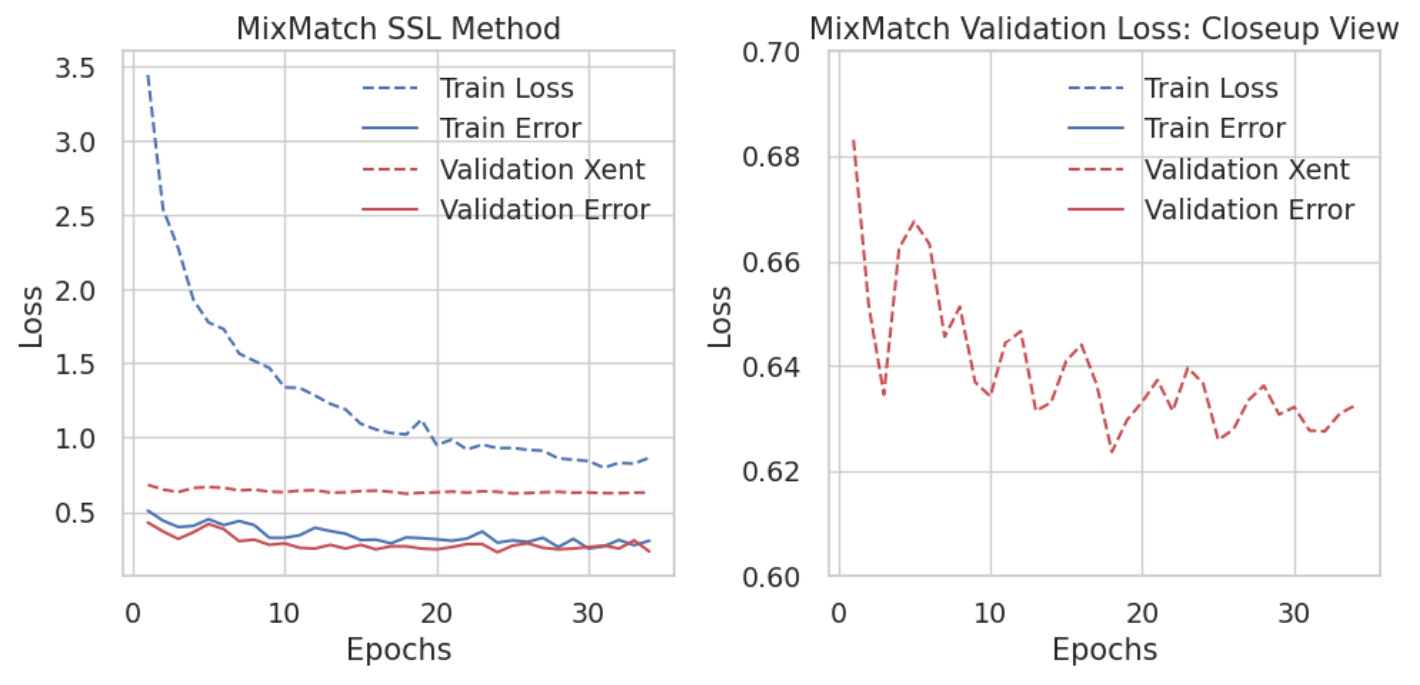
\includegraphics[width=0.5\textwidth]{mixmatch_plots.jpeg}
    \caption{\textbf{Diagnostic plot for MixMatch.}}
    \label{fig:diagnostic_plot}
\end{figure}


Table \ref{table: test_acc_table} summarizes the evaluation results for the tested methods. Our baseline Linear Probing (LP) implementation achieved an accuracy of 88\% on the test dataset, which is within 2\% of the results reported by \cite{awangiskandar2020}. This close match confirms the validity of our implementation and demonstrates the robustness of baseline LP in leveraging pre-trained features for this task.

Fine-Tuning, however, did not yield the expected improvements. Both LP-FT configurations—Fine-Tuning the top 3 and 5 layers—recorded lower accuracies of 84.4\% and 84.0\%, respectively, compared to the baseline LP. This represents a notable drop of approximately 4\%. Diagnostic plots in Figure 1 reveal signs of overfitting during the Fine-Tuning phase: while training loss and error consistently decreased, validation performance plateaued and began to degrade over successive epochs.

We hypothesize that the observed degradation in LP-FT performance stems from the model focusing on spurious patterns in the training data. Specifically, the dataset's low resolution and inherent noise may have caused the model to prioritize features unrelated to the elliptical objects of interest, such as image artifacts, adjacent bright stars, or other irrelevant patterns. These confounding features may have overshadowed the subtle discriminative patterns needed to distinguish True from Rejected PNes, reducing the model’s ability to generalize effectively to the test dataset. This underscores the sensitivity of Fine-Tuning to the quality and characteristics of the training data.

MixMatch pseudo-labeling achieved a test accuracy of 78\%, which was significantly lower than both baseline LP and LP-FT. This is consistent with our hypothesis that MixMatch’s reliance on consistency regularization would struggle with the dataset's low resolution and noisy features. It is reasonable to attribute this to the method's inability to generate reliable pseudo-labels, which in turn limits its capacity to effectively leverage the unlabeled data.
However, based on further preliminary experiments, we believe MixMatch's performance may be improved further if we had incorporated a larger sample of unlabeled data into our dataset. This might suggest that MixMatch may benefit from the additional regularization effect provided by a greater quantity of unlabeled data, even in the presence of unreliable pseudo-labels. Unfortunately, due to time constraints, we were unable to conduct more thorough research and formalize its findings into this report in time.

Overall, our results provide nuanced insights into the application of transfer learning and semi-supervised learning to low-resolution astrophysical datasets. Baseline LP proved to be a robust and reliable method, outperforming both LP-FT and MixMatch. However, the underperformance of LP-FT highlights the need for targeted regularization strategies and advanced preprocessing to mitigate overfitting and prevent the model from focusing on irrelevant features. Similarly, the performance of MixMatch reinforces the importance of dataset quality in enabling semi-supervised approaches to leverage unlabeled data effectively. These findings emphasize the need for method-specific adaptations to overcome the unique challenges posed by specialized, noisy datasets like those used in this study.


\section{Reflection, and Outlook}

\subsection{Take-Home Lessons from Research}

Through this work, we learned several key lessons about our research question and its practical implications:

\textbf{1. Limitations of Small Datasets:}  
One of the takeaways was the impact of having a small labeled dataset. Initially, we aimed to replicate or surpass the results of previous research using a deliberately smaller dataset. While this approach allowed us to experiment with novel methodologies, it quickly became clear that the lack of labeled data limited our ability to achieve the desired results. With access to a larger labeled dataset, we expect that the performance of our approach would improve significantly.

\textbf{2. Overcoming Low-Resolution Artifacts:}  
Another important realization came from dealing with low-resolution images, which introduced artifacts that hindered our model’s performance. In future work, we hypothesize that \textit{a combination of advanced image augmentation techniques and feature transfer from high-resolution images} will help improve the model’s ability to handle artifacts and extract meaningful features from low-resolution data. Addressing these artifacts could improve model generalization and performance in real-world applications.

\subsection{Take-Home Lessons from Implementation and Evaluation}

From an implementation and evaluation perspective, this work reinforced several key insights: 

\textbf{1. The Power of Experimentation with Hyperparameters:}  
Tuning the hyperparameters in our models revealed valuable insights into the behavior of our system. A particularly unexpected finding was the effect of reducing the loss regularization \(\lambda_U\) for unlabeled data in the MixMatch approach, which resulted in an increase in accuracy.

\textbf{2. Managing the Trade-Offs in Resource-Constrained Environments:}  
Implementing this work within the constraints of a limited dataset and computational resources also highlighted an interesting trade-off: while we couldn't achieve the results of larger-scale studies, we were able to develop solutions optimized for resource-constrained environments. This reinforced the importance of being flexible and creative when working within limitations. In future studies, \textit{the key will be to balance innovation with pragmatism}, leveraging available resources in ways that drive meaningful progress despite constraints.

\subsection{Future Outlook}

Moving forward, addressing the limitations identified in this work will be critical to improving performance and advancing the research. Expanding the dataset, experimenting with data augmentation strategies, and exploring more sophisticated models for feature extraction and transfer will be essential next steps. Additionally, continuing to optimize the hyperparameters and fine-tune the model will be crucial for improving performance in real-world applications.

We believe that with more time and resources, our approach has the potential to achieve the accuracy and robustness needed for more widespread adoption within the Deep-space analysis domain, paving the way for even more exploration and application of these techniques in the Astrophysics community.

\newpage
\bibliography{references}

\end{document}
